\documentclass[11pt]{article}
\usepackage[croatian]{babel}  % Croatian typographical rules and hyphenation patterns
\usepackage[utf8]{inputenc}  	% Encoding of Croatian characters
\usepackage[T1]{fontenc}
\usepackage{ae,aecompl}     	% Type 1 fonts, similar to Computer Modern

\usepackage{microtype}				% Improves spacing

\usepackage{booktabs}					% Nice looking tables
\usepackage{enumerate}				% Additional options for listing of items in enumerate environment
\usepackage{algorithm2e}			% Writing pseudo-code
\usepackage{todonotes}				% Adding todo items
\usepackage{dirtree}					% Simple display of directory tree
\usepackage{hyperref}
\usepackage{graphicx}
\usepackage{subfig}
\usepackage{caption}
\usepackage{listings}
\usepackage{enumitem}

\graphicspath{ {./images/} }

\hypersetup{
    colorlinks=true,
    linkcolor=blue,
    filecolor=magenta,
    urlcolor=cyan,
}
\urlstyle{same}
\usepackage{graphics}
\title{
	\Large Sveučilište Josipa Jurja Strossmayera u Osijeku \\
	Fakultet elektrotehnike, računarstva i informacijskih tehnologija \\
	\vspace{4cm}
	\Large Kolegij: Linux u ugradbenim sustavima \\
	\vspace{4cm}
	\Large \textbf{Laboratorijska vježba 2:\\
	Nunchuk - I\textsuperscript{2}C uređaj}
	}
\date{}
\begin{document}
\maketitle
\thispagestyle{empty}
\newpage

\section{Uvod}
Cilj ove vježbe je prepoznati I\textsuperscript{2}C uređaj u operacijskom
sustavu \textit{Linux} te izraditi osnovni \textit{kernel} modul koji će se
nadograđivati u narednim laboratorijskim vježbama. Potrebno je izraditi
stablo uređaja (engl. \textit{device tree}). Također, potrebno je izraditi
kernel modul s osnovnim inačicama \texttt{probe()} i \texttt{remove()} funkcija.

\section{Povezivanje \textit{Nunchuk}-a}
Uzmite \texttt{Nunchuk} uređaj kojeg ste dobili od asistenta.\\
Pomoću konektora ćemo spojiti \texttt{Nunchuk} uređaj na \texttt{J8} pinove
\textit{Raspberry Pi} ploče.\\
Dokumente s korisnim informacijama o Nunchuk uređaju možete preuzeti s adresa:\\
\url{https://bootlin.com/labs/doc/nunchuk.pdf}\\
\url{https://www.robotshop.com/media/files/PDF/inex-zx-nunchuck-datasheet.pdf}\\

\begin{figure}[h!]
\centering
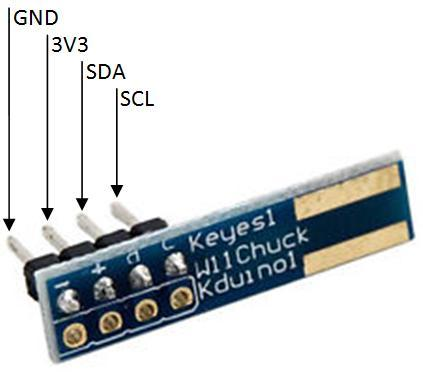
\includegraphics[width=0.4\textwidth]{nunchuk-connector.jpg}
\captionsetup{justification=centering}
\caption{Raspored pinova Nunchuk konektora}
\end{figure}

\begin{figure}[h!]
\centering
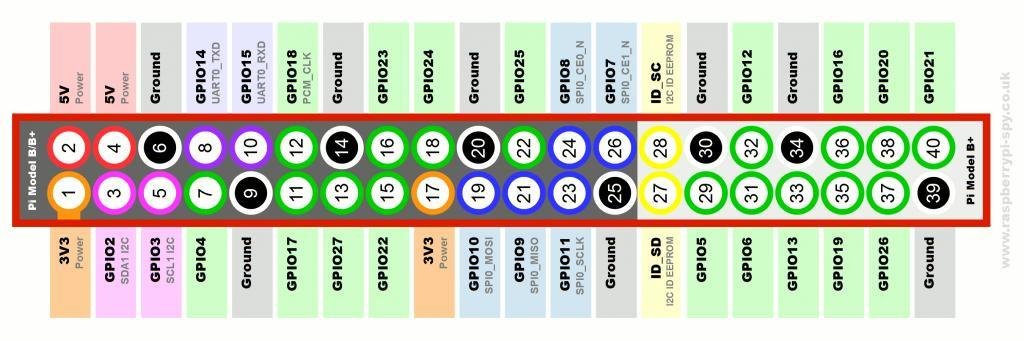
\includegraphics[width=0.95\textwidth]{j8-rpi.jpg}
\captionsetup{justification=centering}
\caption{Raspored pinova J8 konektora na Raspberry Pi 3 ploči}
\end{figure}
\newpage
Sada povežite \textit{Nunchuk} konektor i Raspberry Pi 3 ploču na sljedeći način:
\begin{itemize}
	\item GND pin na J8 pin 9 (GND),
	\item 3V3 pin na J8 pin 1 (3V3),
	\item SCL pin na J8 pin 5 (GPIO3/SCL1 I2C),
	\item SDA pin na J8 pin 3 (GPIO2/SDA1 I2C).
\end{itemize}

\section{Izrada posebnog stabla uređaja (engl. \textit{device tree})}
Da bismo \textit{Linux} jezgri omogućili da rukuje novim uređajem, moramo dodati
opis tog uređaja u stablo uređaja ploče (engl. \textit{board device tree}).
Kako je stablo uređaja za \textit{Raspberry Pi 3} ploču već uključeno u
\textit{Linux} jezgru, mi nećemo raditi izmjene direktno u datoteci koja se već
koristi za ovu ploču nego ćemo napraviti posebno stablo uređaja za našu ploču
s našim uređajem.
\newline
\newline
Pozicionirajte se u Linux izvorni kod koji bi trebao biti na putanji\\
\texttt{/home/rtrk/buildroot/output/build/linux-custom}. Tu se nalazi Linux
izvorni kod pomoću kojega smo stvorili sliku sustava (engl. \textit{image})
za našu \textit{Raspberry Pi} ploču koristeći \texttt{Buildroot} u laboratorijskoj
vježbi 2. Napravite kopiju datoteke \texttt{bcm2710-rpi-3-b.dts} koja se nalazi
u poddirektoriju \texttt{arch/arm/boot/dts} i nazovite ju \texttt{bcm2710-rpi-3-b-custom.dts}.
Napravite u istom direktoriju i izmjene u \texttt{Makefile} datoteci i
omogućite da se i nova \texttt{dts} datoteka kompilira.
\newline
\newline
Unutar nove datoteke, prvo trebamo omogućiti \texttt{i2c1} sabirnicu.
Zatim, deklarirajte \texttt{Nunchuk} uređaj kao čvor nasljednik \texttt{i2ci}.
Odaberite \texttt{nintendo,nunchuk} za \texttt{compatible} postavku.
I\textsuperscript{2}C adresu \texttt{Nunchuk} uređaja možete provjeriti u
\texttt{Nunchuk} dokumentu.
\newline
Nakon potrebnih izmjena \texttt{i2c1} čvor bi trebao izgledati otprilike ovako:
\begin{lstlisting}
&i2c1 {
	pinctrl-names = "default";
	pinctrl-0 = <&i2c1_pins>;
	clock-frequency = <100000>;
	status="okay";

	nunchuk: nunchuk@52 {
		compatible ="nintendo,nunchuk";
		reg = <0x52>;
		status = "okay";
	};
};
\end{lstlisting}
Nakon potrebnih promjena u datoteci stabla uređaja, pozicionirajte se u
korijensku putanju Linux izvornog koda\\
(\texttt{/home/rtrk/buildroot/output/build/linux-custom}).\\
Postavite varijable okruženja potrebne za kompiliranje \texttt{Linux} jezgre:
\begin{lstlisting}
export ARCH=arm
export CROSS_COMPILE=arm-linux-gnueabihf-
\end{lstlisting}
Nakon toga, pokrenite kompiliranje datoteka stabla uređaja koristeći naredbu:
\begin{lstlisting}
make dtbs
\end{lstlisting}
Kopirajte novu \texttt{dtb} datoteku u direktorij \texttt{tftp server}-a
(\texttt{/var/lib/tftpboot} i napravite potrebne izmjene u \texttt{Uboot}
konfiguraciji da bi \textit{Raspberry Pi} ploča prilikom pokretanja učitavala
novu datoteku.
\newline
\newline
Kroz direktorij \texttt{/proc/device-tree} možemo provjeriti sve postavke
stabla uređaja koje je naš sustav učitao.
\newline
\newline
Na primjer, možemo provjeriti prisustvo \texttt{nunchuk} čvora u stablu uređaja:
\begin{lstlisting}
# find /proc/device-tree/ -name "*nunchuk*"
/proc/device-tree/soc/i2c@7e804000/nunchuk@52
\end{lstlisting}
Neke od postavki uređaja možemo pročitati pomoću:
\begin{lstlisting}
cat /proc/device-tree/soc/i2c@7e804000/nunchuk@52/status
\end{lstlisting}

\section{Izrada osnovnog upravljačkog programa za Nunchuk}
Sada možete krenuti s izradom upravljačkog programa za \textit{Nunchuk}.
Unutar direktorija \texttt{/home/rtrk/embedded\_linux/LV3/solutions} stvorite
direktorij imena \texttt{nunchuk}. Unutar tog direktorija stvorite dvije
datoteke: \texttt{nunchuk.c} i \texttt{Makefile}.
\newline
\newline
Struktura \texttt{Makefile} datoteke je standardna. Bitan parametar je
\texttt{KDIR} koji označava putanju do izvornog koda \texttt{Linux} jezgre.
\newline
\newline
\texttt{Makefile} bi trebao izgledati ovako:
\begin{lstlisting}
ifneq ($(KERNELRELEASE),)
obj-m := nunchuk.o
else
KDIR := /home/rtrk/buildroot/output/build/linux-custom
all:
	$(MAKE) -C $(KDIR) M=$$PWD
endif
\end{lstlisting}
Unutar \texttt{nunchuk.c} datoteke treba implementirati sljedeće:
\begin{enumerate}
	\item probe() i remove() funkcije koje će biti pozvane kada je nunchuk
pronađen, odnosno uklonjen. Za sada samo iskoristite poziv printk() unutar
funkcija da biste potvrdili da su funkcije pozvane.
	\item Inicijalizaciju \texttt{i2c\_driver} strukture i registraciju
I\textsuperscript{2}C upravljačkog programa koristeći istu.
koristeći istu. \texttt{compatible} postavke moraju odgovarati onima iz stabla
uređaja.
\end{enumerate}
\newpage
Sadržaj \texttt{nunchuk.c} datoteke bi mogao biti ovakav:
\begin{lstlisting}
#include <linux/init.h>
#include <linux/module.h>
#include <linux/i2c.h>

static int
probe(struct i2c_client *client,
		const struct i2c_device_id *id)
{
	printk(KERN_ALERT "nunchuk probe() is called\n");
	return 0;
}

static int
remove(struct i2c_client *client)
{
	printk(KERN_ALERT "nunchuk remove() ic called\n");
	return 0;
}

static const struct i2c_device_id id[] = {
	{"nunchuk", 0},
	{},
};
MODULE_DEVICE_TABLE(i2c, id);

static struct of_device_id nunchuk_dt_match[] = {
	{.compatible = "nintendo,nunchuk",},
	{ },
};

static struct i2c_driver nunchuk_driver = {
	.driver = {
		.name = "nunchuk",
		.owner = THIS_MODULE,
		.of_match_table = nunchuk_dt_match,
	},
	.probe = probe,
	.remove = remove,
	.id_table = id,
};

module_i2c_driver(nunchuk_driver);
MODULE_LICENSE("GPL");
\end{lstlisting}

Pokrenite prevođenje (prethodno moraju biti postavljene varijable okruženja
\texttt{ARCH} i \texttt{CROSS\_COMPILE}!!!) koristeći naredbu:
\begin{lstlisting}
make
\end{lstlisting}

Stvoreni \texttt{nunchuk.ko} kernel modul kopirajte na \texttt{NFS} putanje
od ploče \texttt{/home/rtrk/embedded\_linux/LV2/solutions/nfsroot/root}.
Učitajte i uklonite kernel modul koristeći naredbe \texttt{insmod} i \texttt{rmmod}.

\end{document}
